
% decide i dont need overview  \subsection{Overview}
% To delineate the development of structure--function coupling (SFC) from birth to age five, we analyzed multimodal MRI data from the Baby Connectome Project ($N= [Insert N]$, age 0--5 years)\cite{howellUNCUMNBaby2019}. We defined vertex-wise SFC as the Pearson correlation between a region's structural connectivity (SC) strength and its functional connectivity (FC) profile (Methods).

% We first characterized global developmental trends. Averaged across the cortex, SFC, intracortical myelination (T1w/T2w ratio), and excitation--inhibition balance (indexed by the Hurst exponent, $H$) all exhibited robust age-related changes (Fig.~\ref{fig:timeline}a). From birth to five years, mean SFC increased by approximately 23\%, indicating a progressive alignment of functional signals with underlying structural architecture. Concurrently, intracortical myelin increased by $\sim$15\%, while the Hurst exponent decreased by $\sim$6\%, reflecting a global shift toward higher excitation--inhibition (E/I) ratios and faster neural dynamics. These trajectories persisted after controlling for sex, motion, and site effects (Fig.~\ref{fig:timeline}b), establishing that early childhood is defined by three concurrent macro-scale trends: strengthening structure--function alignment, microstructural maturation, and the remodeling of cortical temporal dynamics.

\subsection{OSSVD improve performance of fMRI and individual gradient}
% Placeholder: denoising result details will be added later.
\begin{figure}[t]
  \centering
  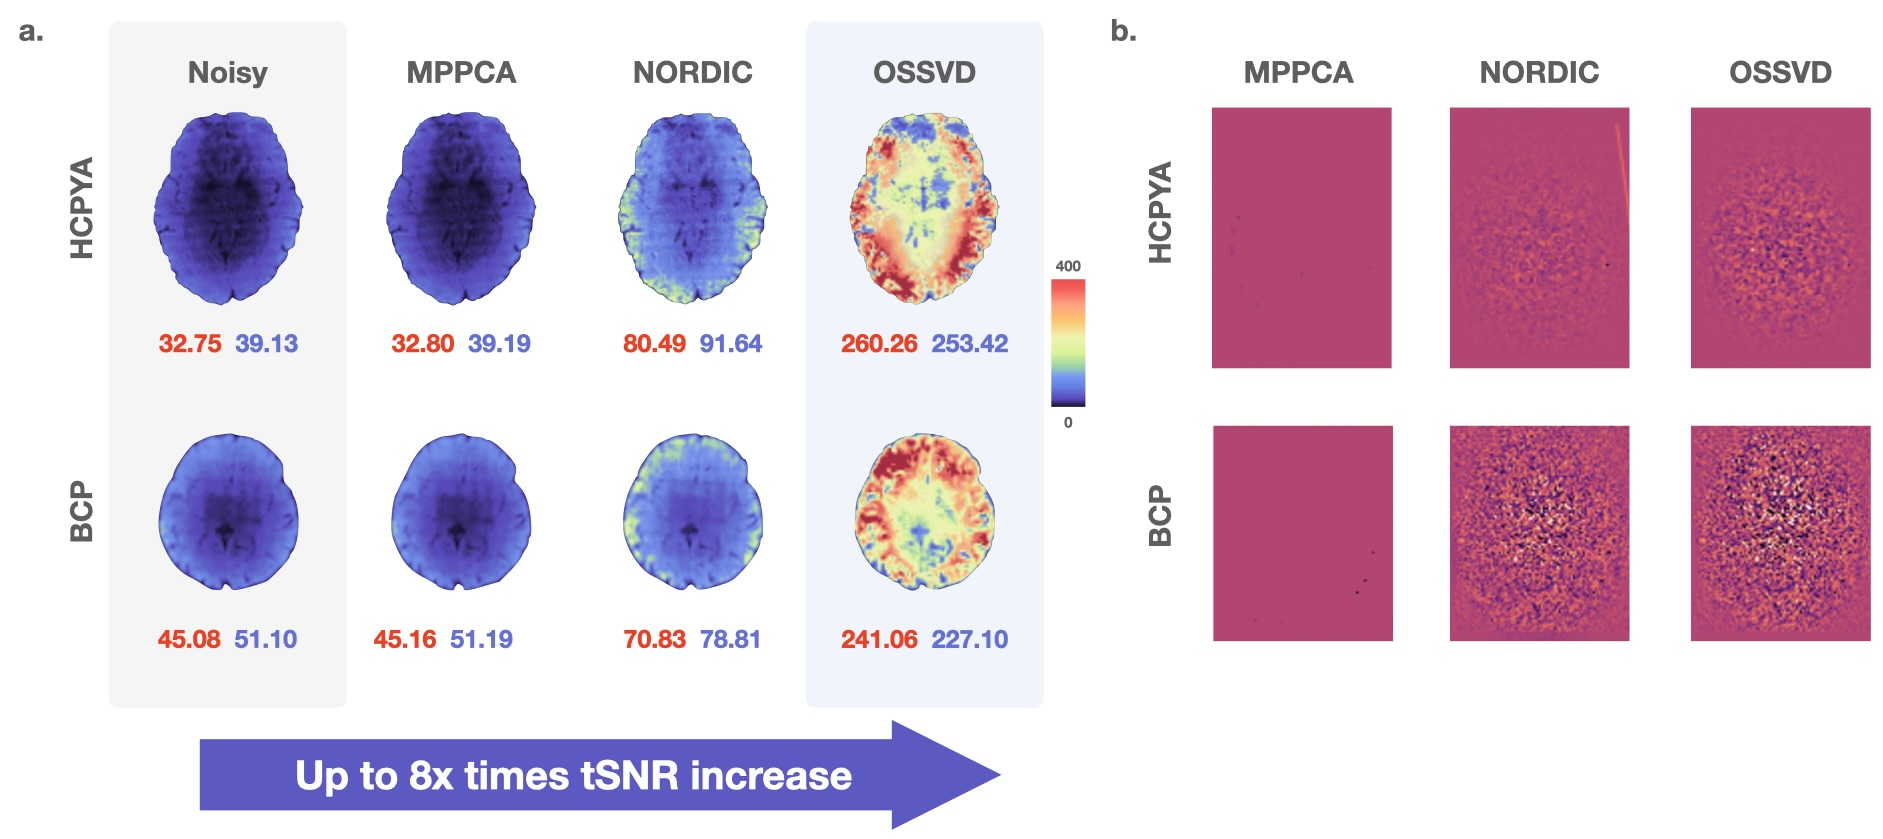
\includegraphics[width=0.95\linewidth]{figure/Figure7_denoisingresult.jpeg}
  \caption{\textbf{$|$ Effects of noise removal.} (a) Temporal signal-to-noise ratio (tSNR) before and after denoising. OS-SVD achieves the largest tSNR improvement, particularly in gray matter, and outperforms MP-PCA and NORDIC. (b) Residual maps show no discernible loss of structural information after denoising.}
  \label{fig:denoising_result}
\end{figure}

\begin{figure}[t]
  \centering
  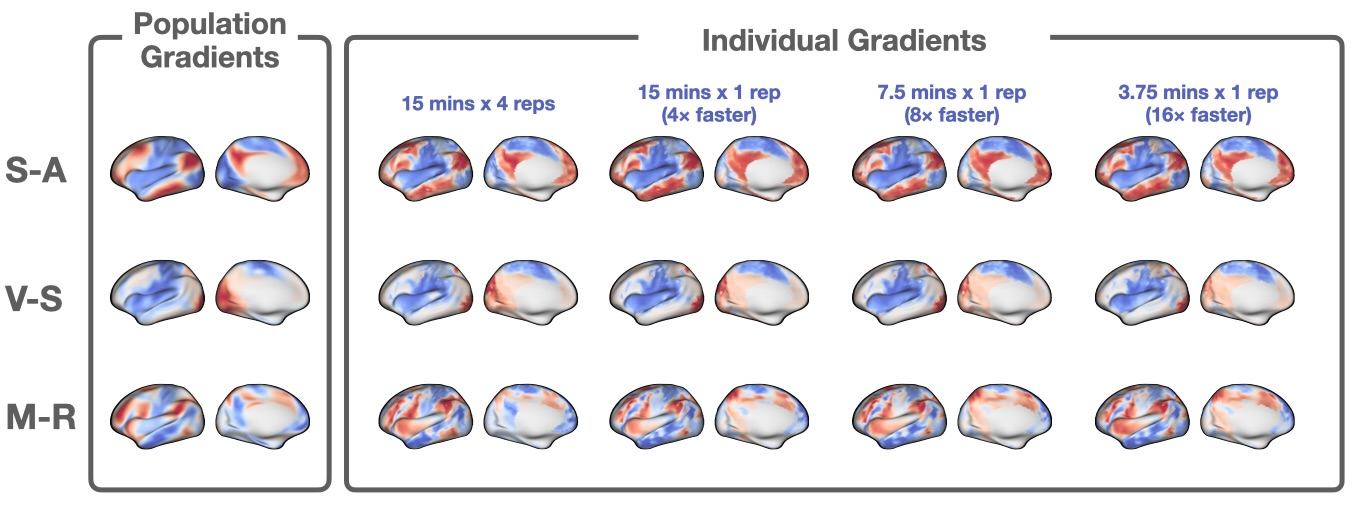
\includegraphics[width=0.95\linewidth]{figure/Figure8_gradientcomparison.jpeg}
  \caption{\textbf{$|$ Effects of using fewer volumes and repetitions on gradients.}
  OS-SVD preserves gradient patterns even with less than 4 minutes of data, reducing acquisition time by 16 times.}
  \label{fig:denoising_gradient_comparison}
\end{figure}

Denoising efficiency and structural preservation: OS-SVD denoising increases temporal SNR by 8 times, particularly in gray matter, significantly outperforming MP-PCA by 800\% and NORDIC by 300\% (Fig.~\ref{fig:denoising_result}a). Both OS-SVD and NORDIC produce residual maps with no discernible structural features, indicating that only noise is removed (Fig.~\ref{fig:denoising_result}b). MP-PCA yields an almost zero residual map, consistent with ineffective noise removal in this dataset.

Denoising effect on individual gradients: Denoising significantly enhances individual gradients in both adult and infant fMRI (Fig.~\ref{fig:denoising_gradient_comparison}). Without denoising, individual gradients show dispersed patterns with abrupt spatial changes, especially in higher-order gradients. OS-SVD produces smooth individual gradients, with spatial patterns that closely match the S--A (somatosensory--association), V--S (visual--sensorimotor), and M--R (modulation--representation) axes observed in population-level results.

Acceleration with temporally undersampled data: We evaluated OS-SVD's ability to produce high-quality gradients from temporally undersampled data to reduce acquisition time (Fig.~\ref{fig:denoising_gradient_comparison}). Four rs-fMRI scans per subject (1200 volumes, 15 minutes per scan, 1 hour total) were used for diffusion embedding. We then tested OS-SVD using only one scan (4x faster), with reduced volume counts of 600 (8x faster) and 300 (16x faster). With denoising, reducing volume count and scan number did not compromise gradient quality. Three principal functional connectome axes remained detectable with data acquired in under 4 minutes.

% figure 2
\subsection{Functional gradient differentiation in HBCD and BCP during early infancy}

We focused on the sensorimotor--association (S--A) gradient, which captures the primary axis of functional hierarchy from primary sensorimotor to high-order association cortices, and the visual--somatomotor (V--S) gradient, which captures a key secondary axis separating visual processing from somatomotor functions. Both functional gradients showed increasing differentiation over the first 6 months of life (Figs.~\ref{fig:gradient_timeline_bcp} and \ref{fig:gradient_timeline_hbcd}). Vertex-wise GAMMs showed divergent age-related trends at the gradient poles for both gradients, indicating that contrast between the poles increases over time. The S--A gradient showed the strongest developmental change at the primary sensorimotor pole, while the V--S gradient showed peak changes at the visual cortex pole. Association regions consistently exhibited weaker or negative effects, confirming the overall increasing gradient differentiation. These developmental patterns align with the known hierarchical organization observed in the adult brain.

To compare cross-cohort consistency, we examined gradient trajectories in both the HBCD cohort (0--6 months) and age-overlapping BCP data. The direction of change was concordant across cohorts, with early differentiation concentrated at unimodal poles and weaker change in association cortex (Figs.~\ref{fig:gradient_timeline_bcp} and \ref{fig:gradient_timeline_hbcd}), indicating that the emergence of functional hierarchy during the first postnatal months is reproducible across independent infant datasets.

\begin{figure}[t]
  \centering
  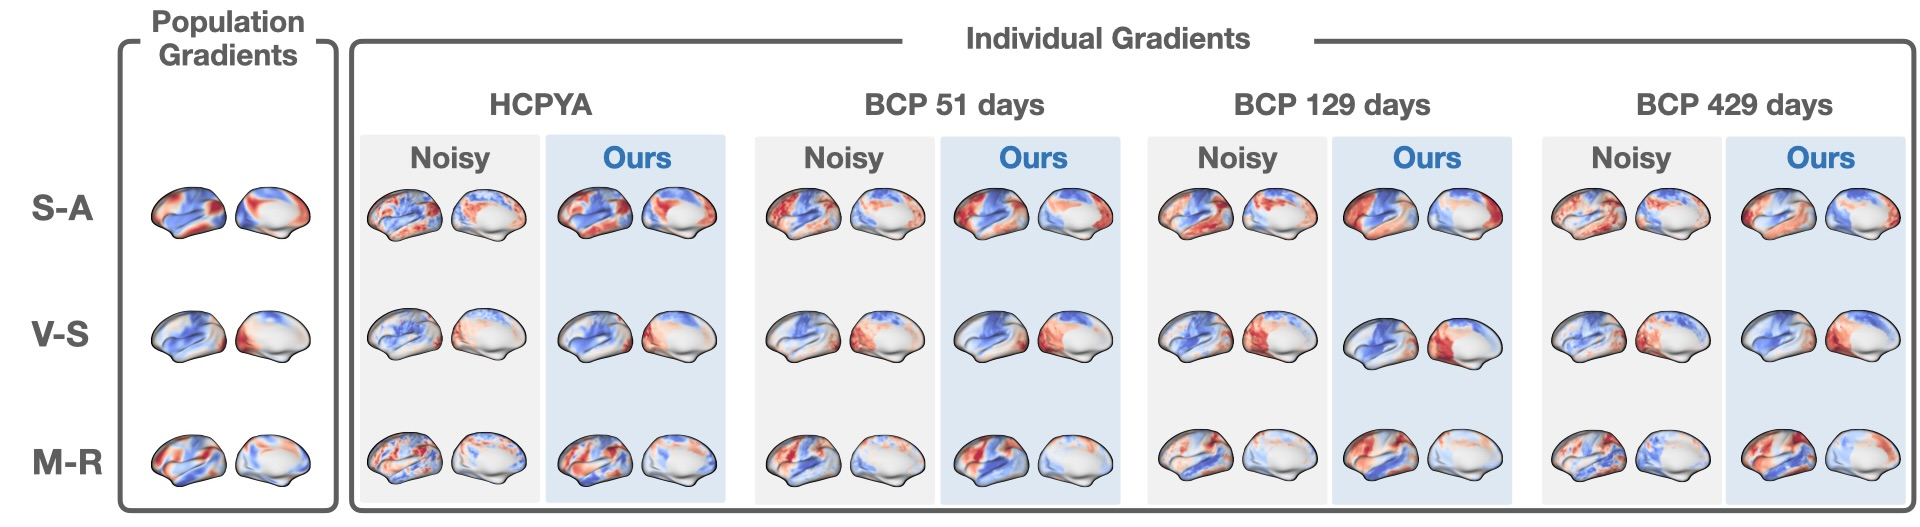
\includegraphics[width=0.95\linewidth]{figure/Figure9_gradienttimeline_BCP.jpeg}
  \caption{\textbf{$|$ Early-infant maturation of functional gradients in BCP.}
  Developmental trajectories of S--A and V--S gradients in the BCP cohort (51, 129, and 429 days) show increasing pole-to-pole differentiation, with strongest effects at primary sensorimotor and visual poles and weaker effects in association cortex.}
  \label{fig:gradient_timeline_bcp}
\end{figure}

\begin{figure}[t]
  \centering
  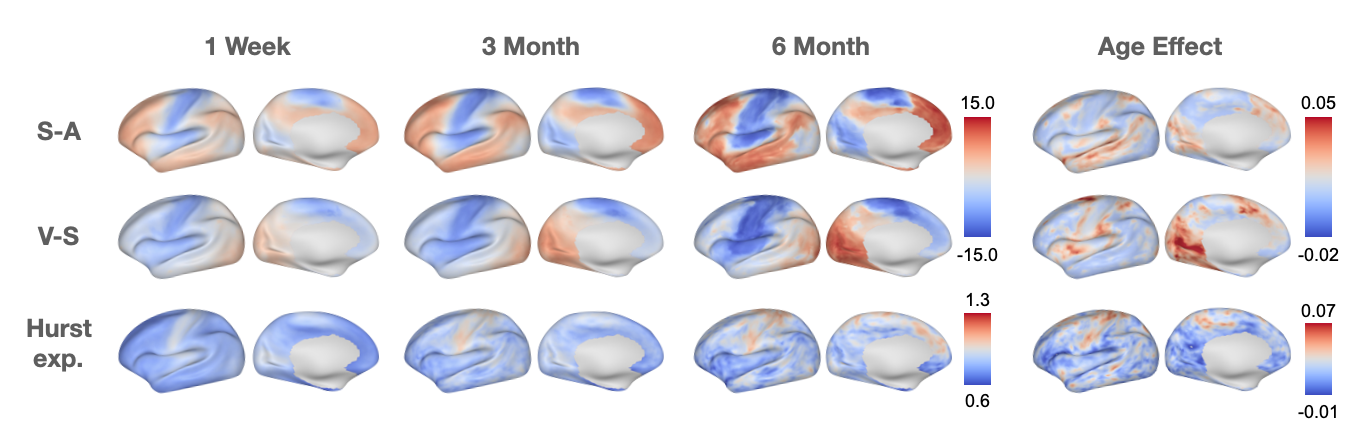
\includegraphics[width=0.95\linewidth]{figure/Figure10_gradienttimeline_HBCD.png}
  \caption{\textbf{$|$ Early-infant maturation of functional gradients in HBCD.}
  Developmental trajectories of S--A and V--S gradients during the first postnatal months show increasing pole-to-pole differentiation, with strongest effects at primary sensorimotor and visual poles and weaker effects in association cortex.}
  \label{fig:gradient_timeline_hbcd}
\end{figure}

% figure 3
\subsection{Global strengthening of structure--function coupling, myelination and temporal dynamics from birth to five years}

To characterize how structure-function coupling (SFC) and its substrates change across early childhood, we first quantified cortex-wide age trajectories for SFC, intracortical myelination, and excitation-inhibition (E/I)-related dynamics. Using multimodal MRI data from the Baby Connectome Project (BCP; $N = 221$ subjects, $372 scans$, $0$--$5$ years)\cite{howellUNCUMNBaby2019}, we computed vertex-wise SFC as the Pearson correlation between each vertex's structural connectivity (SC) and functional connectivity (FC) profiles (Methods). Intracortical myelination was indexed by the T1w/T2w ratio, and local temporal dynamics were summarized by the Hurst exponent ($H$), a scale-free measure of autocorrelation that inversely relates to the E/I ratio. Developmental change in each metric was modeled with generalized additive mixed models (GAMMs), allowing flexible nonlinear trajectories while accounting for repeated measures within individuals.

\begin{figure}[t]
  \centering
  \includegraphics[width=0.95\linewidth]{figure/Figure11_timeline.pdf}
  \caption{\textbf{$|$ Developmental trajectories of SFC, Hurst exponent, and myelination across early childhood.}
  Vertex-level cortical maps show GAMM-fitted trajectories from birth to 5 years, highlighting coordinated but regionally heterogeneous maturation of structure-function coupling, excitation-inhibition-related dynamics, and intracortical myelination.}
  \label{fig:timeline}
\end{figure}

Averaged across the cortical surface, all three measures showed pronounced age-related change from birth to five years (Fig.~\ref{fig:timeline}). Mean SFC increased by approximately $\sim\!23\%$, indicating a progressive tightening of the correspondence between functional interactions and underlying structural architecture. Over the same period, intracortical myelination increased by roughly $\sim\!15\%$, reflecting rapid maturation of the white-matter scaffold that supports long-range communication, whereas the mean Hurst exponent decreased by about $\sim\!6\%$, consistent with a global shift toward faster, more desynchronized dynamics and higher E/I ratios. These global trends remained robust after adjusting for sex, head motion and imaging site (Methods), establishing early childhood as a period of coordinated strengthening of structure--function alignment, microstructural maturation, and temporal reconfiguration.

Cortical surface maps at representative ages further revealed that these global trajectories are not spatially homogeneous (Fig.~\ref{fig:timeline}). Even in this coarse view, sensorimotor regions exhibited higher SFC and myelin and lower $H$ earlier in life, whereas association cortices showed weaker initial coupling, lower myelin, and more slowly declining $H$. These observations suggest that hierarchical differences in maturation are already apparent at the macroscale and motivate a more detailed analysis of how the sensorimotor--association axis organizes the timing and form of SFC, SC, FC, myelination and E/I development.

% \subsection{Network hierarchy constrains SFC magnitude and maturation with  structural and functional connectivity}
% Having established that structure--function coupling, myelination and temporal dynamics all change markedly from birth to five years, we next examined how this global strengthening is distributed across canonical functional networks from a vertex-wise resolution. Vertex-wise BOLD timeseries and diffusion tractography were used to construct individual $20{,}484 \times 20{,}484$ FC and SC matrices, from which we derived vertex-wise SFC and mapped it onto the cortical surface (Fig.~\ref{fig:SFC_atlas}a). The group-averaged FC and SC matrices, sorted by these networks, showed a strongly modular architecture with dense within-network and weaker between-network connectivity, particularly for unimodal VIS and SMN systems (Fig.~\ref{fig:SFC_atlas}b). Chord diagrams of FC and SC intra-network connections emphasized this organization, with strong bidirectional coupling among unimodal and attentional networks and comparatively sparser connectivity involving limbic cortex (Fig.~\ref{fig:SFC_atlas}c).
% SFC followed a rigid hierarchical organization: coupling was strongest in unimodal visual (VIS) and somatomotor (SMN) networks, intermediate in the dorsal/ventral attention (DAN/VAN) and frontoparietal (FP) networks, and weakest in the limbic (LIM) system (Fig.~\ref{fig:SFC_atlas}a). This hierarchy mirrors the underlying connectivity strengths, as violin plots of these distributions revealed that networks with high SFC also exhibited the strongest intra-network SC and FC (Extended Data Fig.~\ref{fig:supplementary_net_violin}), whereas transmodal networks with weaker internal SC/FC—especially LIM and DMN—displayed reduced SFC.
% Conversely, transmodal networks with weaker internal SC/FC—especially limbic and default mode cortex—displayed reduced SFC, consistent with greater functional flexibility and looser structural constraints. Thus, regions that are heavily wired and functionally cohesive exhibit the tightest constraints of structure on function.

% Developmental trajectories varied systematically by network. Longitudinal vertex-wise surface maps revealed that SFC increases from birth through five years across much of the cortex, with the largest age-related gains in association territories and relatively smaller changes in primary sensory and motor regions (Fig.~\ref{fig:SFC_atlas}e, top). The corresponding maps of temporal SFC variance showed decreasing variance in unimodal cortex but more heterogeneous changes in higher-order networks, suggesting early stabilization of SFC in sensory systems and prolonged reconfiguration in association cortex (Fig.~\ref{fig:SFC_atlas}e, bottom). Together, these findings indicate that a common network hierarchy shapes the magnitude and maturation of vertex-wise SC, FC and SFC: unimodal systems are strongly wired and tightly structure-function coupled from early in life, whereas transmodal systems remain more weakly coupled but undergo extended refinement throughout early childhood.


% We next asked whether the hierarchical organization observed across canonical networks reflects a more continuous gradient of maturation along the sensorimotor-association (S-A) axis. Therefore, we projected vertex-wise SC, FC and SFC dynamics onto the continuous sensorimotor-association (S-A) axis, the principal gradient of cortical organization\cite{sydnorNeurodevelopmentAssociationCortices2021}. Aligning vertices from sensorimotor (S-end) to association (A-end) revealed that hierarchical position strongly predicts developmental timing (Fig.~\ref{fig:SFC_sa}).  

% xrref
%Zero-centered SFC trajectories diverged along the axis: sensorimotor regions began with relatively high coupling that stabilized or slightly decreased, whereas association regions started with lower coupling that increased robustly over time (Fig.~\ref{fig:SFC_sa}a). Examining SC and FC in the same S--A bins clarified these SFC trends (Fig.~\ref{fig:SFC_sa}b,c). At the association (A) end, both SC and FC strength increased over early childhood, with their age-related gains closely aligned. As a result, the correlation between SC and FC profiles strengthened, yielding steadily rising SFC values in high-rank bins. In contrast, at the sensorimotor (S) end, SC increased rapidly but FC tended to become more selective and, in some cases, decrease relative to the global mean. This early mismatch in the direction of SC and FC change reduced their profile correlation, producing the observed drop in SFC despite growing structural strength.
% Quantifying the rate of change (first derivative) and curvature (second derivative) confirmed a gradient of plasticity (Fig.~\ref{fig:SFC_sa}d-i). Sensorimotor bins showed large positive SC slopes but weaker or even negative FC slopes early in life, yielding modest or negative SFC first derivatives. Association bins, by contrast, displayed jointly positive SC and FC slopes, which translated into robust positive SFC first derivatives that persisted across the 0-5 year window. Bin-averaged SFC first derivatives increased with S--A rank (Spearman's $\rho \approx 0.6$, $p < 0.001$; Fig.~\ref{fig:SFC_sa}f), mirroring the shift from SC-FC mismatch at the S-end to SC-FC co-growth at the A-end. Downsampling the full $20{,}484 \times 20{,}484$ SC and FC matrices into $20 \times 20$ S-A-ordered blocks confirmed that connections involving association vertices carried the largest positive age derivatives in both modalities (Fig.~\ref{fig:SFC_sa}e), consistent with a hierarchy of joint structural and functional strengthening.
% Second-derivative analyses highlighted corresponding differences in curvature (Fig.~\ref{fig:SFC_sa}g,h). In sensorimotor bins, SC second derivatives were near zero or slightly negative, and FC derivatives shifted from negative toward zero, yielding predominantly negative or flat SFC second derivatives—concave-down trajectories that rise early and then decelerate. In association bins, both SC and FC second derivatives remained positive for longer, indicating sustained acceleration in structural and functional strengthening; SFC second derivatives showed the same pattern, with increasingly concave-up trajectories along the S--A axis. Together, these results demonstrate that the S--A gradient serves as a common coordinate system for the co-development of SC, FC and SFC: early-maturing sensorimotor cortex is characterized by rapid structural growth and FC refinement that temporarily reduce SC–FC correlation, whereas later-maturing association cortex shows joint structural and functional strengthening that drives progressive increases in structure--function coupling.


\subsection{From vertices to networks: SC, FC and SFC converge on a common S-A hierarchy}

\begin{figure}[t]
  \centering
  \includegraphics[width=0.95\linewidth]{figure/Figure12_SFC_atlas.pdf}
  \caption{\textbf{$|$ Atlas-level structure--function coupling (SFC).}
  Vertex, parcel, and network-level representations of SC, FC, and SFC highlighting hierarchical organization across cortical systems.}
  \label{fig:SFC_atlas}
\end{figure}

\begin{figure}[t]
  \centering
  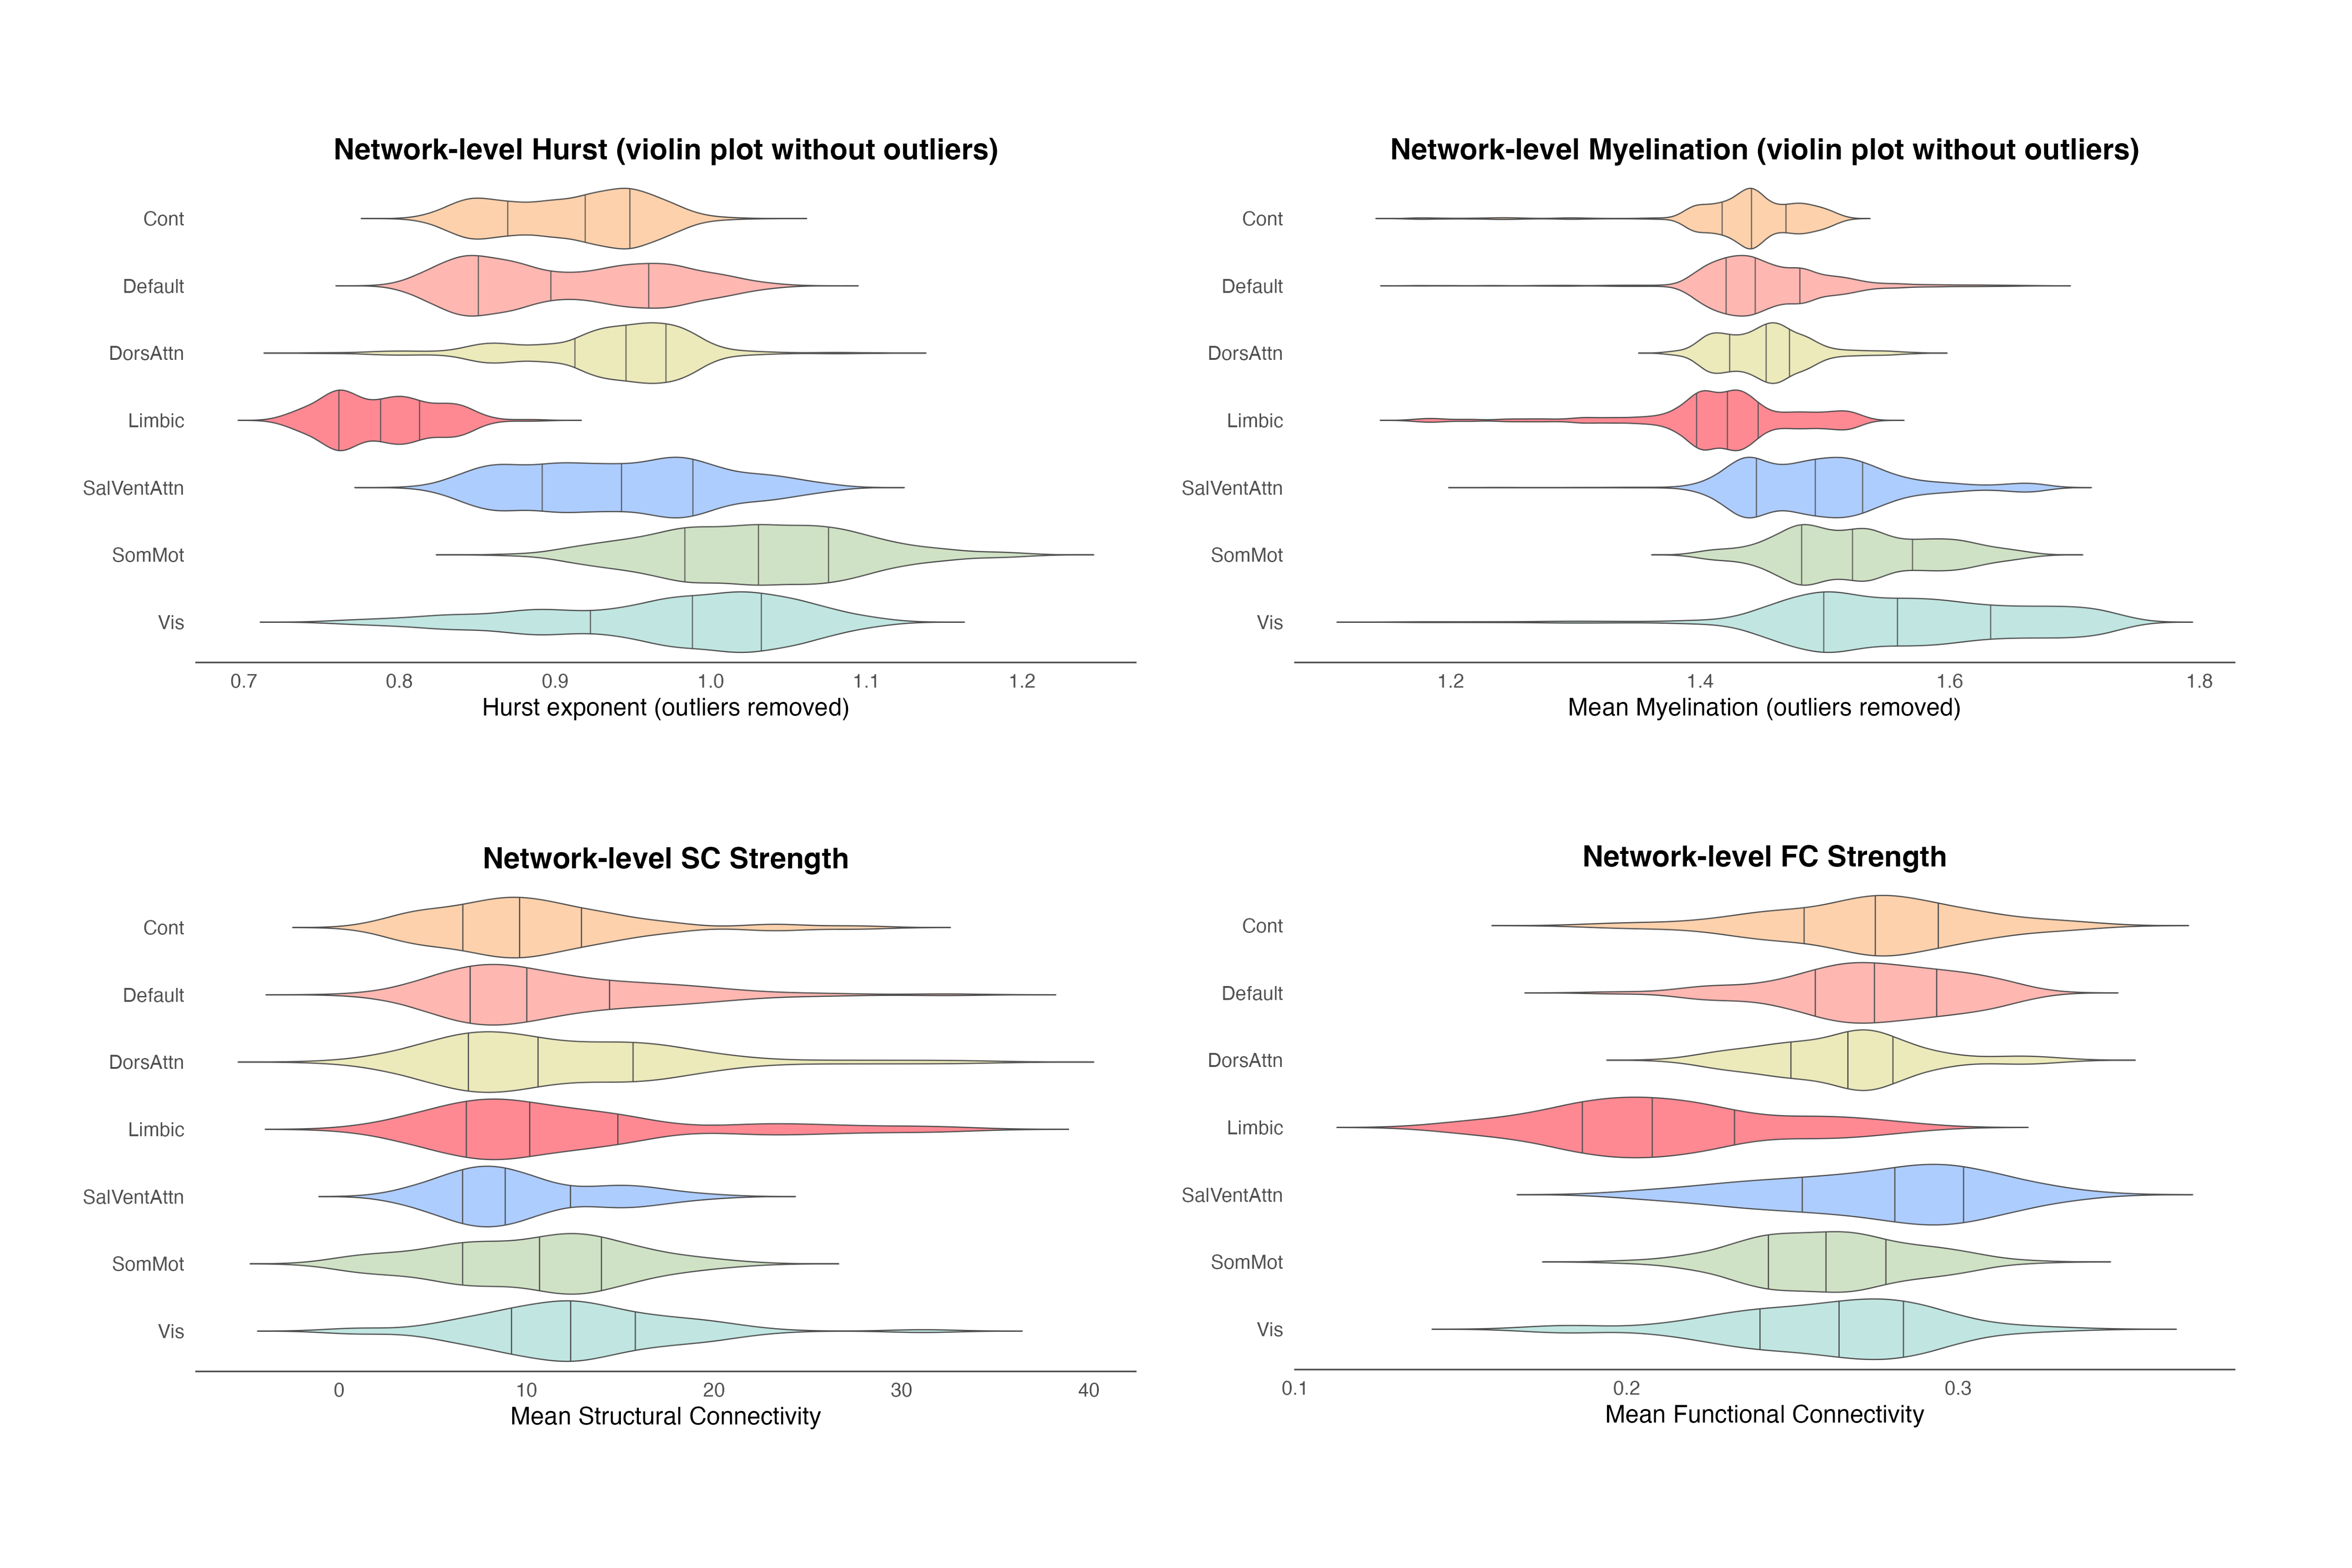
\includegraphics[width=0.95\linewidth]{figure/Figure13_supplementary_net_violin.pdf}
  \caption{\textbf{$|$ Supplementary network-level distributions of SC, FC, and SFC.}
  Violin distributions across canonical networks show stronger intra-network coupling in unimodal systems and weaker coupling in transmodal systems.}
  \label{fig:supplementary_net_violin}
\end{figure}

We defined SC, FC and SFC at the vertex level by constructing individual $20{,}484 \times 20{,}484$ SC and FC matrices from diffusion tractography and vertex-wise BOLD time series for each individual. Next, we derived vertex-wise SFC before mapping all three measures onto the cortical surface (Fig.~\ref{fig:SFC_atlas}a). We then examined the results at three spatial scales---vertices, 400-level ROI, and canonical 7-network partitions---and found that SC, FC and SFC displayed a strikingly homogeneous organization across scales. Group-averaged SC and FC matrices, sorted by canonical networks, exhibited a strongly modular architecture with dense within-network and weaker between-network connectivity, most prominently in unimodal visual (VIS) and somatomotor (SMN) systems (Fig.~\ref{fig:SFC_atlas}b). Chord diagrams of intra-network connections emphasized this pattern, revealing robust reciprocal coupling among unimodal and attentional networks and comparatively sparse connectivity involving limbic cortex (Fig.~\ref{fig:SFC_atlas}c). Longitudinal plots further showed that the strength of these positive intra-network connections increased over infancy and early childhood, with the steepest gains occurring around the first year of life and plateauing thereafter (Extended Data Fig.~\ref{fig:supplementary_FC_Developmental_Trajectory}).

\begin{figure}[t]
  \centering
  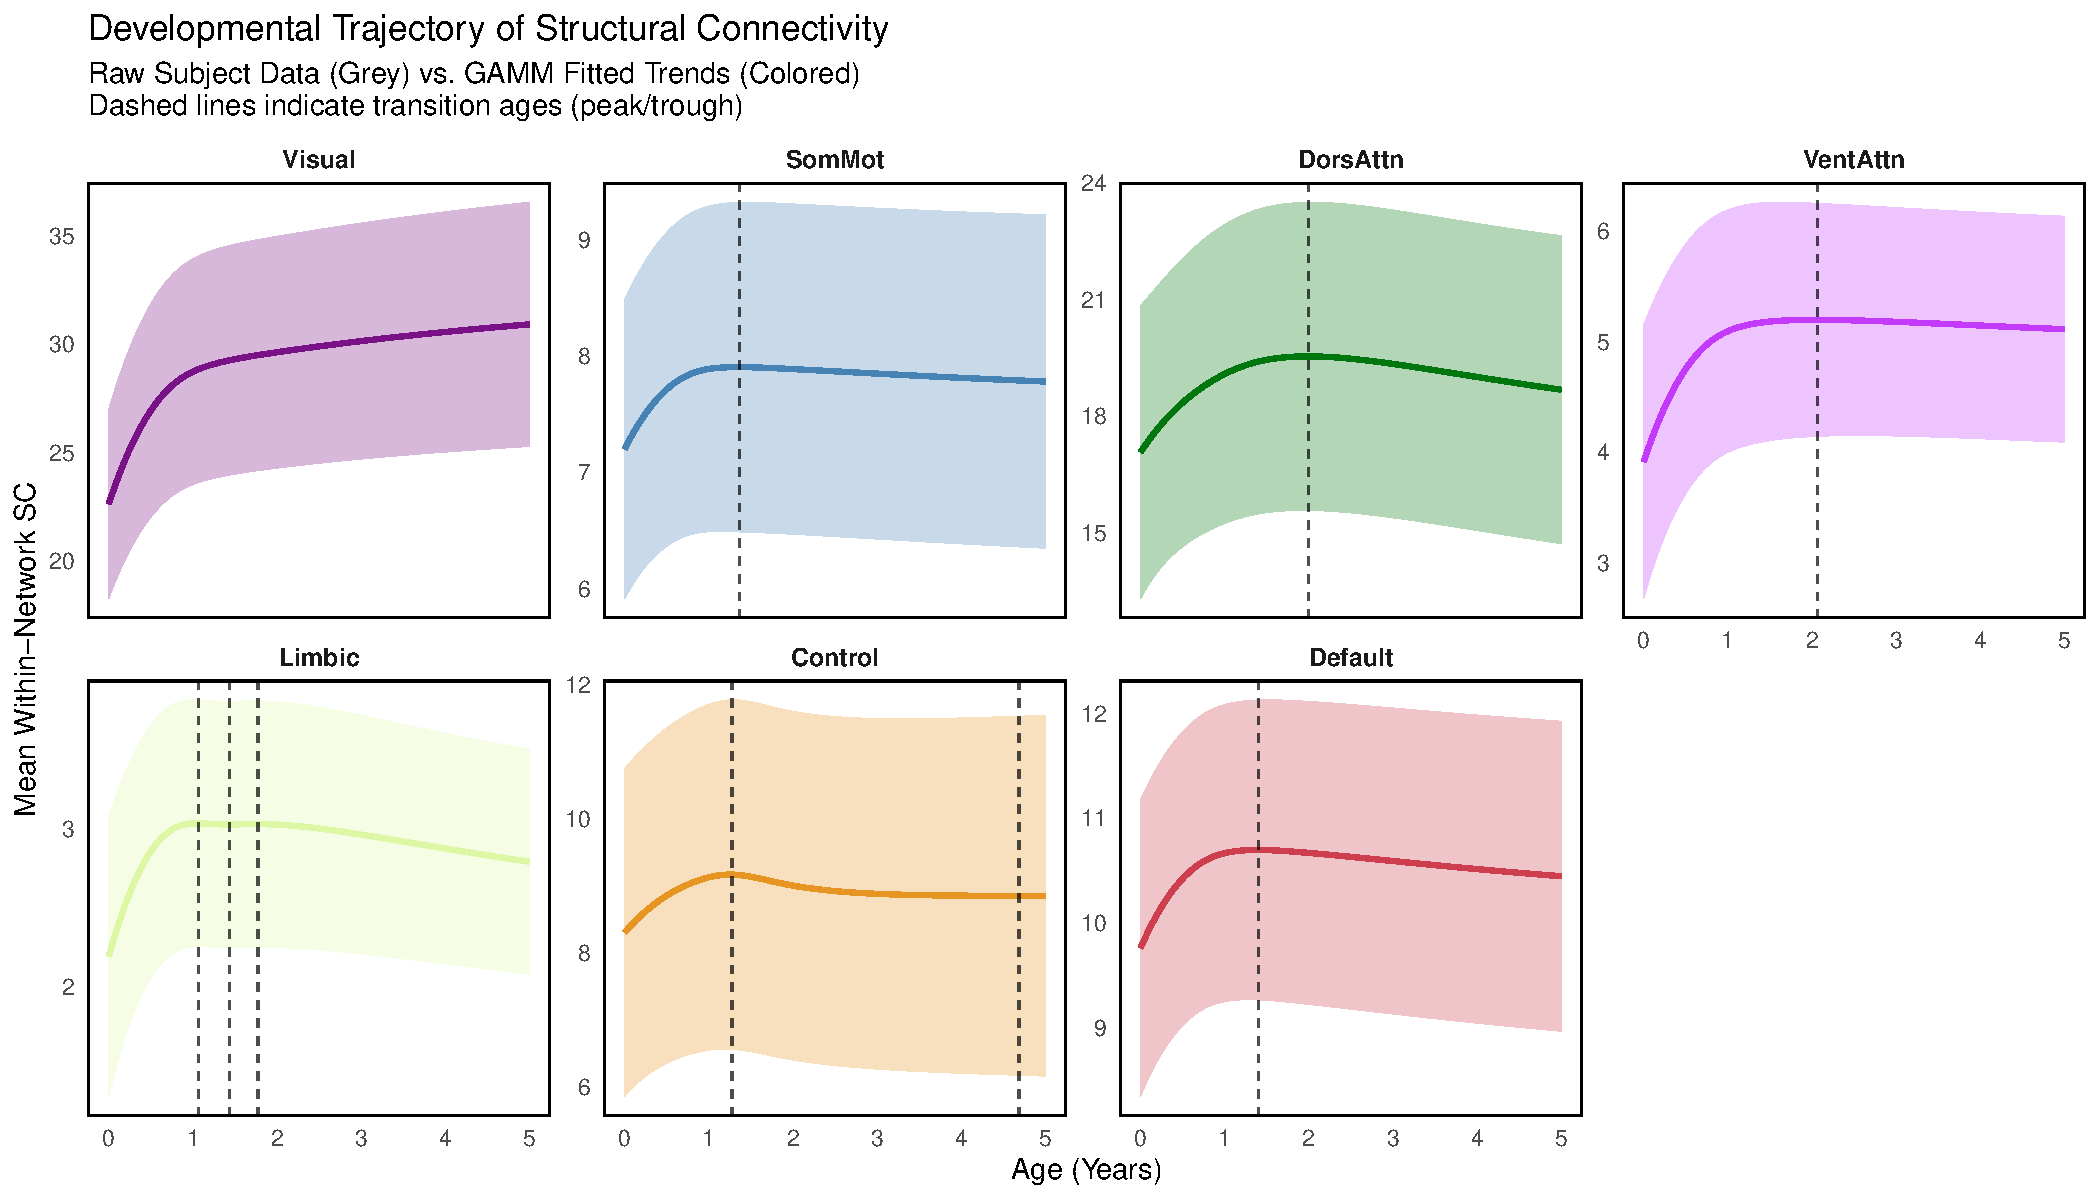
\includegraphics[width=0.95\linewidth]{figure/Figure14_SC_Developmental_Trajectory.pdf}
  \caption{\textbf{$|$ Developmental trajectory of structural connectivity (SC).}
  Longitudinal SC trends across early childhood highlight age-dependent strengthening of structural connections.}
  \label{fig:sc_developmental_trajectory}
\end{figure}

\begin{figure}[t]
  \centering
  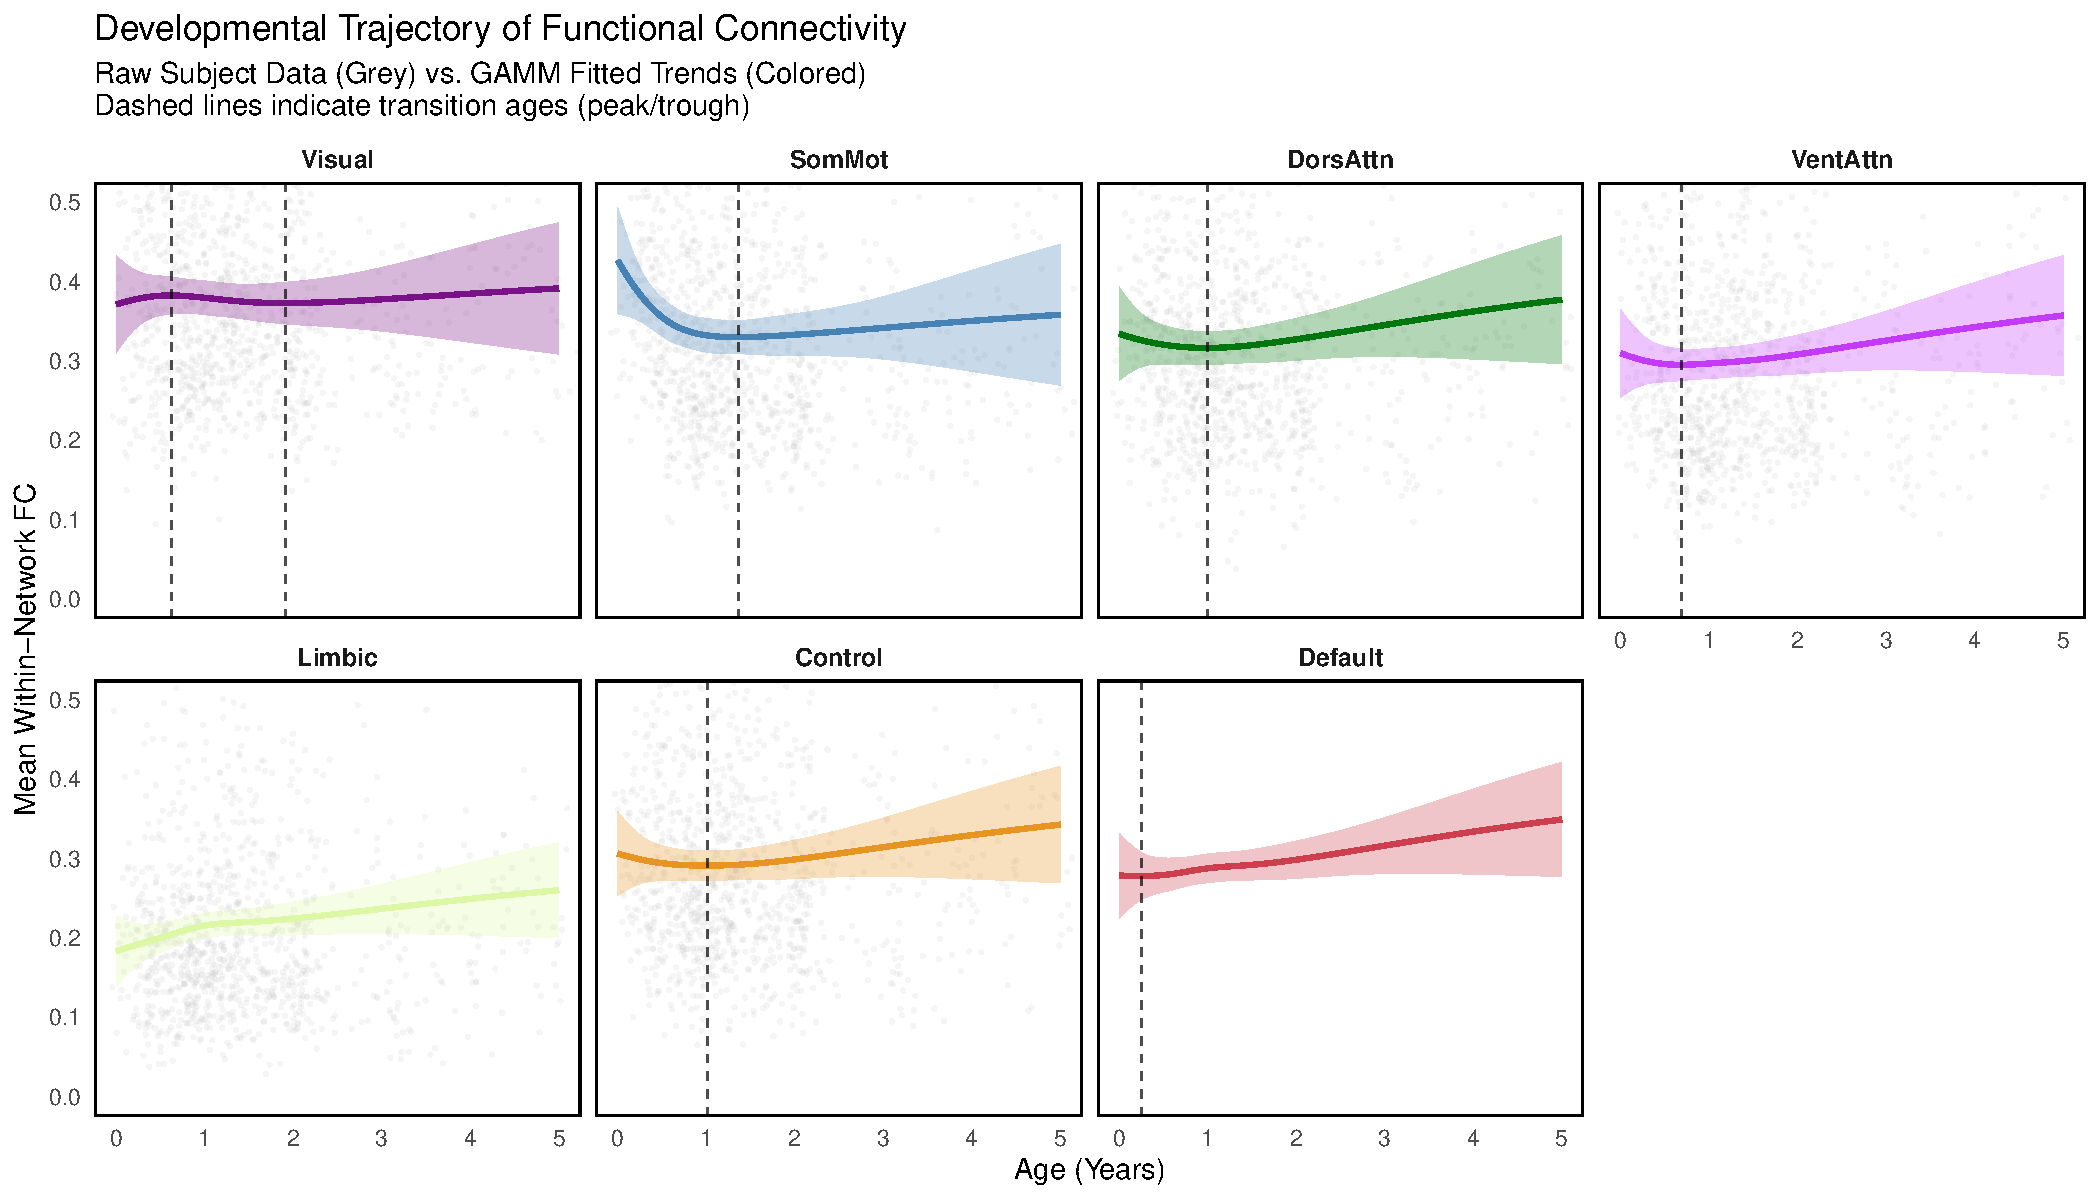
\includegraphics[width=0.95\linewidth]{figure/Figure15_FC_Developmental_trajectory_intra.pdf}
  \caption{\textbf{$|$ Intra-network developmental trajectory of functional connectivity (FC).}
  Longitudinal intra-network FC trends show maturation-related changes in functional coupling across systems.}
  \label{fig:fc_developmental_trajectory_intra}
  \label{fig:supplementary_FC_Developmental_Trajectory}
\end{figure}

Within this modular scaffold, SFC followed a rigid hierarchy. Coupling was strongest in unimodal VIS and SMN networks, intermediate in dorsal and ventral attention (DAN/VAN) and frontoparietal (FP) networks, and weakest in limbic (LIM) and default mode (DMN) systems (Fig.~\ref{fig:SFC_atlas}a). Violin plots of vertex-wise distributions showed that networks with high SFC also had the strongest intra-network SC and FC, whereas transmodal networks with weaker internal SC/FC---especially LIM and DMN---displayed reduced SFC (Extended Data Fig.~\ref{fig:supplementary_net_violin}). Thus, regions that are heavily wired and functionally cohesive exhibit the tightest structure-function alignment, whereas transmodal systems remain more loosely constrained.

Developmentally, this hierarchy was preserved but its magnitude evolved systematically along the S--A axis. Vertex-wise age models revealed widespread increases in SFC from birth to five years, with relatively modest changes in primary sensory and motor regions and marked gains in association cortex (Fig.~\ref{fig:SFC_atlas}e, top). Temporal SFC variance decreased in unimodal cortex but showed more heterogeneous patterns in higher-order networks, consistent with early stabilization of coupling in sensory systems and prolonged reconfiguration in association regions (Fig.~\ref{fig:SFC_atlas}e, bottom). Projecting vertex-wise SC, FC and SFC trajectories onto the continuous S--A gradient clarified these effects (Fig.~\ref{fig:SFC_sa}). Zero-centred SFC trajectories diverged along the axis: sensorimotor vertices began with relatively high coupling that stabilized or slightly declined, whereas association vertices started lower and increased robustly over time (Fig.~\ref{fig:SFC_sa}a). Examining SC and FC within the same S--A bins showed that, at the association (A) end, both SC and FC strengths increased in concert, yielding steadily rising SFC and large positive first derivatives (Fig.~\ref{fig:SFC_sa}b--f). At the sensorimotor (S) end, SC increased rapidly but FC became more selective and, in some cases, decreased relative to the global mean, producing an early mismatch in SC and FC change and modest or negative SFC derivatives. Downsampling the full $20{,}484 \times 20{,}484$ SC and FC matrices into $20 \times 20$ S--A-ordered blocks confirmed that connections involving association vertices carried the largest positive age derivatives in both modalities (Fig.~\ref{fig:SFC_sa}e). Second-derivative analyses further indicated concave-down trajectories (early rise then deceleration) in sensorimotor cortex and more prolonged concave-up trajectories (sustained acceleration) in association cortex (Fig.~\ref{fig:SFC_sa}g--i). Together, these results show that the S--A hierarchy provides a shared coordinate system for the co-development of SC, FC and SFC. Early-maturing sensorimotor cortex is strongly wired and tightly coupled from the outset, whereas later-maturing association cortex undergoes joint structural and functional strengthening that drives progressive increases in structure--function coupling throughout early childhood.

\begin{figure}[t]
  \centering
  \includegraphics[width=0.95\linewidth]{figure/Figure16_SFC_sa.pdf}
  \caption{\textbf{$|$ SFC trajectories along the sensorimotor--association axis.}
  SA-ordered analyses show hierarchical differences in SFC baseline, slope, and curvature from birth to early childhood.}
  \label{fig:SFC_sa}
\end{figure}

\subsection{Excitation--inhibition balance shapes the SFC landscape via temporal dynamics}

\subsubsection{Gradient--E/I coupling (HBCD results)}
The Hurst exponent decreased significantly across the cortex from 1 week to 6 months, with the largest decreases in sensorimotor and visual regions, spatially overlapping with areas of strongest gradient maturation. Network-level analyses confirmed that somatomotor and visual networks exhibited the highest within-network variance, reflecting heterogeneous E/I development (Fig.~\ref{fig:hurstgradient_hbcd}a). GAMM-fitted trajectories revealed a sharp initial decline in Hurst exponent across all networks, with the steepest decrease occurring in the first 6 weeks. The first derivative showed peak acceleration around 6 weeks, followed by stabilization at approximately 3 months (Fig.~\ref{fig:hurstgradient_hbcd}c). Functional gradient maturation was spatially coupled with shifts in local E/I balance. Vertex-wise analyses revealed negative correlations between Hurst exponent and both S--A (\(r = -0.335\)) and V--S (\(r = -0.289\)) gradients: regions at the primary ends of both gradients exhibited lower Hurst values, indicating higher E/I ratio. This coupling strengthened over development, with correlation slopes becoming steeper by 6 months (Fig.~\ref{fig:hurstgradient_hbcd}b). Regions showing the strongest gradient differentiation also exhibited the largest Hurst decreases.

These findings demonstrate that functional gradient differentiation and excitation-inhibition dynamics are spatially coupled during early infancy, with primary sensory regions showing both the strongest gradient maturation and the largest shifts toward excitation dominance. This coupling suggests that local physiological changes in E/I balance may drive the emergence of macroscale functional organization. The developmental trajectory follows a sensorimotor-first pattern: primary regions differentiate rapidly in the first 6 weeks before stabilizing, while association cortices lag behind, consistent with hierarchical models of cortical maturation. Our vertex-level framework, combining functional gradient analysis with Hurst exponent mapping, enables fine-scale characterization of neurophysiology in the infant brain. Applied to the HBCD cohort, this approach establishes normative trajectories of gradient--E/I coupling that may facilitate early detection of atypical patterns implicated in neurodevelopmental disorders. As longitudinal HBCD data become available, this framework will enable tracking of individual developmental trajectories across infancy.

\begin{figure}[t]
  \centering
  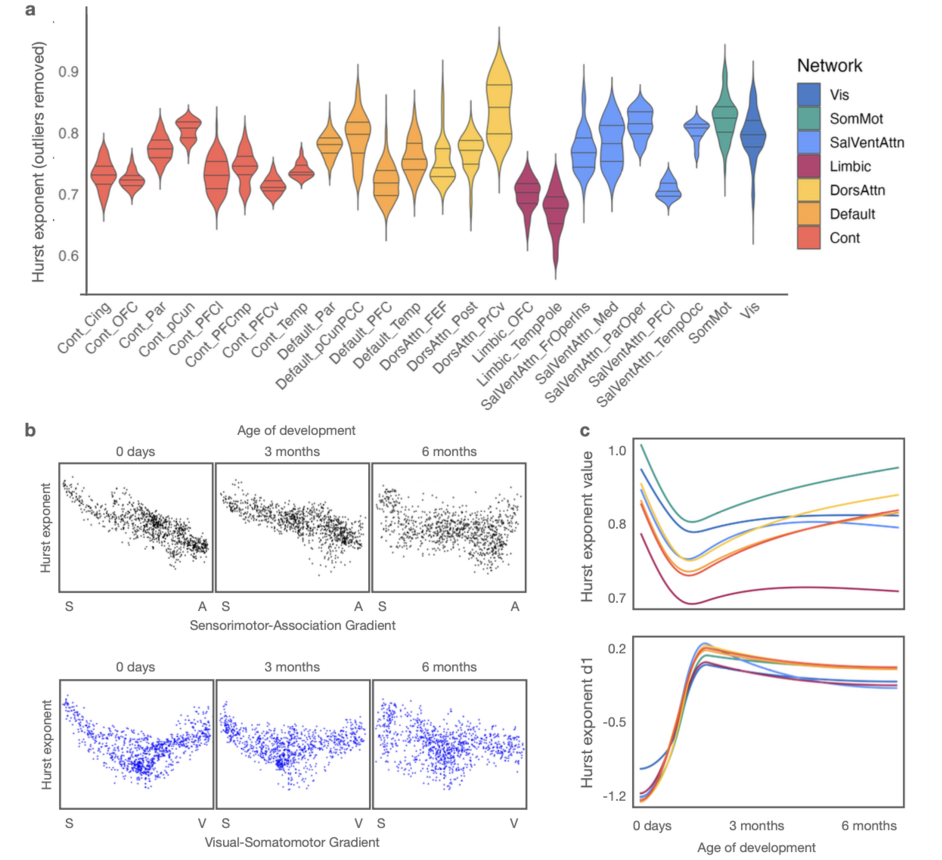
\includegraphics[width=0.95\linewidth]{figure/Figure17_Hurstgradient_HBCD.png}
  \caption{\textbf{$|$ Network-level organization and dynamics of E/I balance across early postnatal development.}
  (a) Hurst exponent distributions across Schaefer 400 parcels. Primary networks (visual, somatomotor) show higher average Hurst values, suggesting relatively lower excitation--inhibition (E/I) balance. (b) Scatter plots showing the relationship between functional gradients (SA, VS) and Hurst exponent across development. At each age point, 1,000 vertices were randomly sampled from the cortical surface (10k mesh). A negative association emerges and strengthens with age, particularly at the sensorimotor and visual ends of each gradient. (c) Top: Network-averaged Hurst exponent trajectories over the first 6 months of life. Bottom: First derivative of Hurst exponent over age, showing peak rate of change at $\sim$6 weeks across all networks, with strongest early decline in primary systems.}
  \label{fig:hurstgradient_hbcd}
\end{figure}

\begin{figure}[t]
  \centering
  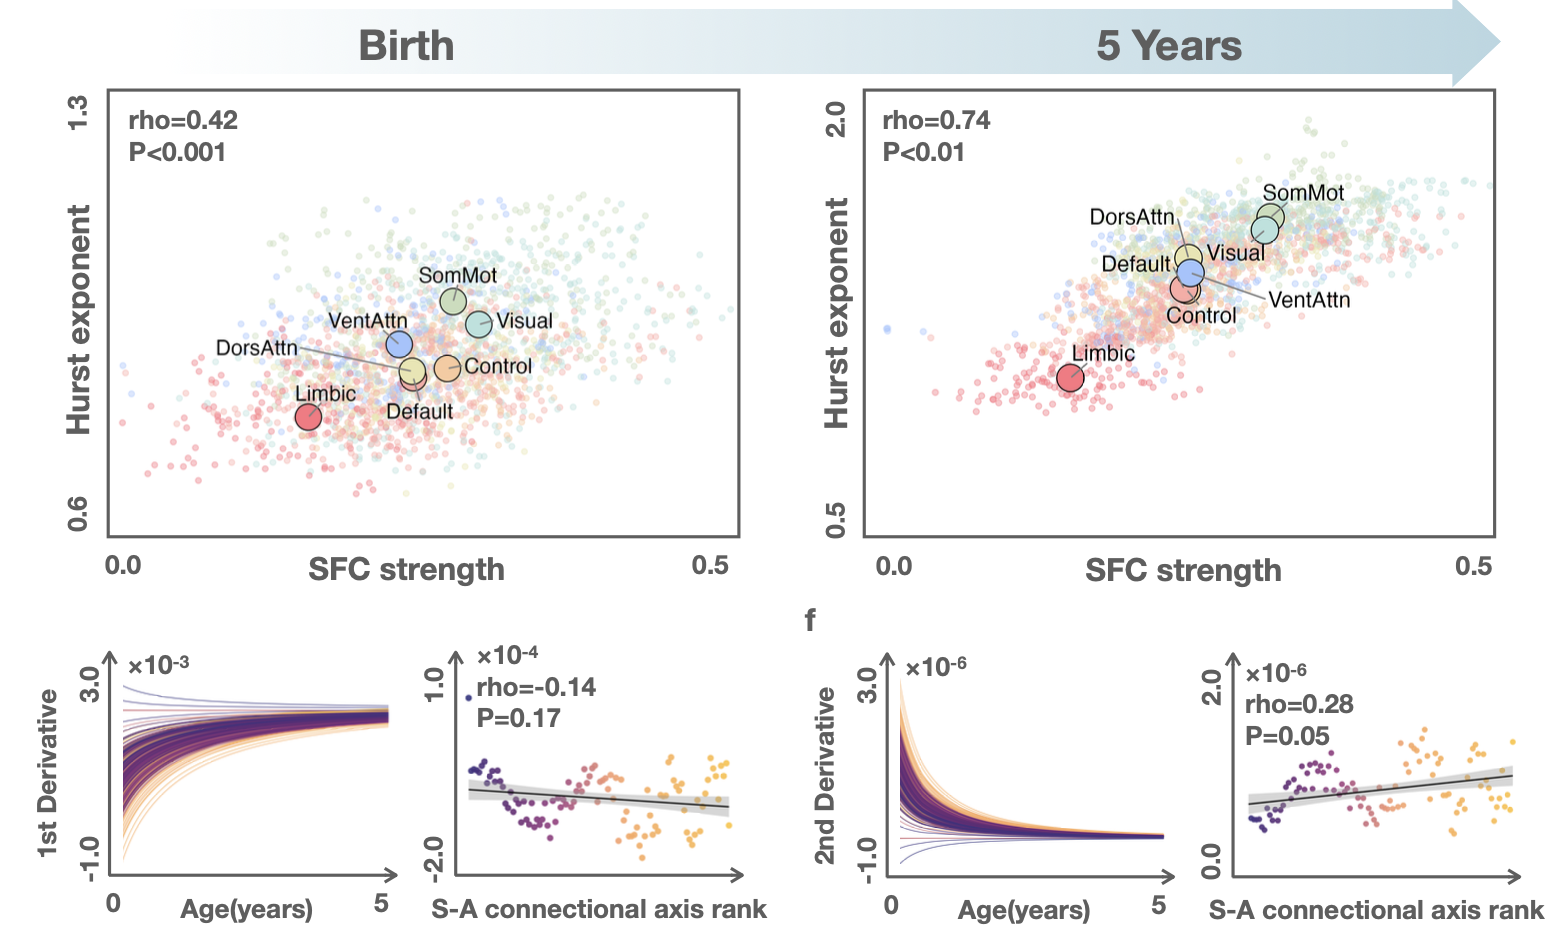
\includegraphics[width=0.95\linewidth]{figure/Figure18_Hurstsa_BCP.png}
  \caption{\textbf{$|$ Hurst trajectory along the S--A axis in BCP.}
  Developmental patterns of Hurst exponent along the sensorimotor--association hierarchy in the BCP cohort.}
  \label{fig:hurstsa_bcp}
  \label{fig:Hurst_sa}
  \label{fig:hurst_sa}
\end{figure}

We next asked how local temporal dynamics contribute to the emergence of structure-function coupling. For each subject and vertex, we estimated the Hurst exponent ($H$) of the resting-state BOLD signal on the cortical surface, using it as a proxy for excitation-inhibition (E/I) balance, where lower $H$ reflects faster, more stochastic dynamics (higher E/I ratio) and higher $H$ reflects slower, more autocorrelated dynamics (lower E/I ratio). Across 0 to 5 years, mean $H$ declined globally, indicating a developmental shift toward higher E/I ratios, with earlier stabilization in sensorimotor cortex and more prolonged, nonlinear change in transmodal association regions (Fig.~\ref{fig:Hurst_sa}a–d). To relate these trajectories to the sensorimotor-association (S-A) hierarchy, we projected an established S–A gradient onto the infant cortical surface by matching each vertex to an adult template and then grouping vertices into 100 equally sized bins along the gradient (purple = lowest S-end, yellow = highest A-end). For each bin, we computed the mean first and second derivatives of the fitted $H$ curves across 0 to 5 years; plotting these 100 bin averages yielded the SA-ordered line and scatter plots in Fig.~\ref{fig:Hurst_sa}e,f. Curvature of $H$ trajectories varied systematically along the axis (second derivative vs.\ S-A rank, Spearman's $\rho \approx 0.28$, $p \approx 0.05$; Fig.~\ref{fig:Hurst_sa}f), consistent with extended remodeling of temporal dynamics in association cortex.

We then examined how the spatial coupling between $H$ and SFC strengthens over development. At birth, the vertex-wise scatter of SFC versus $H$ was broad and diffuse, with only a modest positive relationship and considerable overlap across networks. By age five, points clustered tightly along a steeper positive trend, and the network centroids followed a clear hierarchy: primary visual and somatomotor systems showed the highest SFC and $H$, followed by attention and control networks, with limbic and default mode regions occupying the low-SFC, low-$H$ end of the continuum. Correspondingly, the spatial correlation between mean SFC and mean $H$ increased from infancy to preschool ($\rho_{\text{birth}} \approx [0.42]$ to $\rho_{\text{5y}} \approx [0.74]$), indicating that regions that maintain slower, more autocorrelated dynamics increasingly become the ones whose functional coupling most closely tracks structural wiring. This association remained robust after accounting for position along the S-A axis and intracortical myelination (partial Spearman’s $\rho \approx 0.56$, $p < 10^{-4}$), suggesting that E/I-related temporal regimes provide a functional component that independently shapes how tightly structure and function are coupled during early childhood.


\subsection{Intracortical myelination tracks the emergence of SFC}
We also found that structural maturation (intracortical myelination), indexed by the T1w/T2w ratio, helps explain this hierarchical pattern of SFC during the first 5 years of life. Myelination in sensorimotor cortex exhibited rapid, early-saturating increases, whereas association cortex showed slower but more sustained growth across the 0–5 year window (Fig.~\ref{fig:myelin_sa}c–f). First-derivative analyses confirmed steeper early myelin gains in low-rank (sensorimotor) regions and more prolonged increases in high-rank (association) regions (Spearman’s $\rho \approx 0.57$, $p < 0.001$; Fig.~\ref{fig:myelin_sa}e), consistent with classic myelogenetic sequences.

\begin{figure}[t]
  \centering
  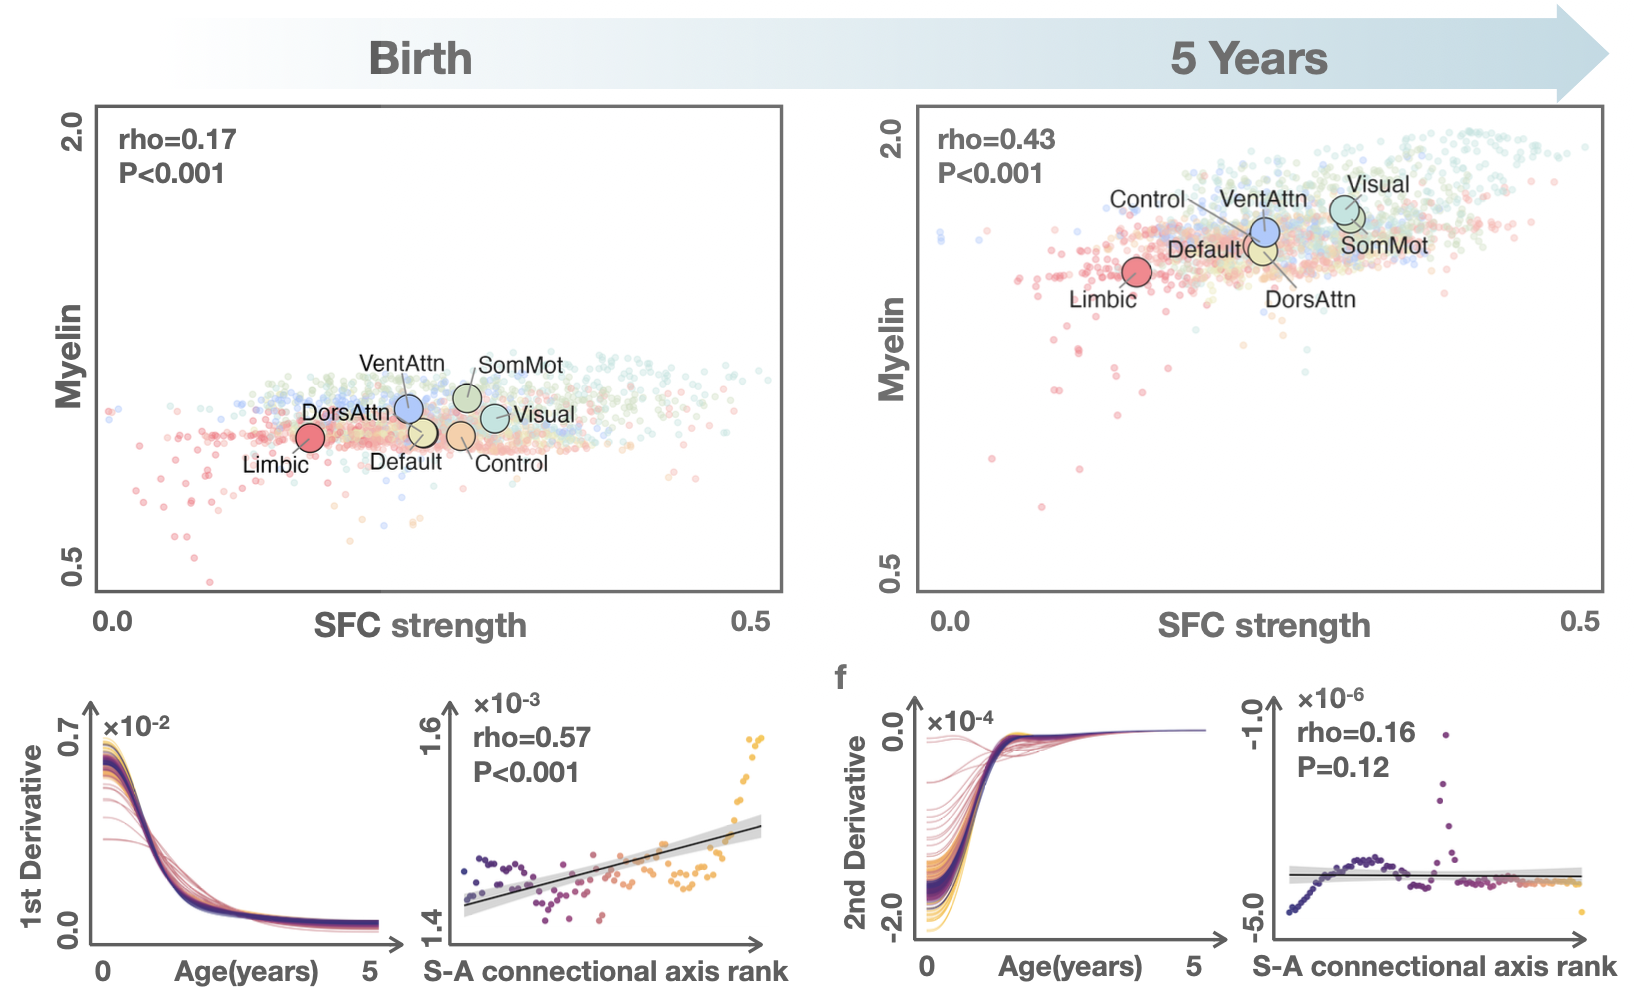
\includegraphics[width=0.95\linewidth]{figure/Figure19_myelinsa_BCP.png}
  \caption{\textbf{$|$ Myelination trajectory along the S--A axis in BCP.}
  Developmental pattern of intracortical myelination along the sensorimotor--association hierarchy in early childhood.}
  \label{fig:myelinsa_bcp}
  \label{fig:myelin_sa}
\end{figure}

Spatial coupling between myelination and SFC strengthened over development, but with a different profile than for $H$. At birth, SFC–myelin scatterplots showed only weak alignment, with considerable dispersion and limited separation across networks. By age five, points became more tightly distributed around a positive regression line, and network means fell into a familiar hierarchy: unimodal visual and somatomotor systems again occupied the high-myelin, high-SFC end, attentional and control networks were intermediate, and limbic/default regions remained low on both axes. The corresponding vertex-wise correlation between SFC and myelin increased from early infancy to preschool ($\rho_{\text{birth}} \approx [0.17]$ to $\rho_{\text{5y}} \approx [0.43]$), indicating that as the cortical scaffold matures, regions with denser intracortical myelin are increasingly those in which functional interactions most closely follow structural connectivity.

In conclusion, this SFC-myelin relationship partly reflects shared organization along the S-A axis and with E/I-related dynamics, but myelin also explains unique variance. After controlling for S-A rank and $H$, the spatial association between SFC and myelin remained significant, albeit attenuated (partial Spearman's $\rho \approx 0.18$, $p < 10^{-4}$). Together with the Hurst findings, these results support a dual-component view in which intracortical myelination supplies a slowly evolving structural scaffold, while E/I-related temporal regimes provide a functional constraint; the intersection of these two components determines where, and how strongly, cortical structure and function become locked together during early childhood.



\subsection{Microstructure and excitation--inhibition balance gate how SC and FC co-development expresses as SFC}

Finally, we asked how the co-development of structural and functional connectivity along the S--A axis is shaped by local microstructure and neural dynamics. Because SFC is defined as the correlation between each vertex's SC and FC profiles, its maturation should depend not only on how strongly SC and FC grow, but also on whether this growth occurs in a microcircuit context that favors stable, structurally constrained dynamics. We therefore related vertex-wise SFC to intracortical myelination (T1w/T2w) and the Hurst exponent, both in space and in time, leveraging the same vertex-level maps used in the SA and network analyses (Figs.~\ref{fig:timeline}, \ref{fig:myelin_sa}, \ref{fig:hurst_sa}).

Across the cortical sheet, SFC was strongly coupled to intracortical myelination: vertices with higher T1w/T2w ratios exhibited systematically stronger SFC (Spearman's $r = 0.658$, $p < 0.001$). A similarly strong spatial relationship was observed between SFC and the Hurst exponent: regions with higher H (more temporally autocorrelated, inhibitory-like dynamics) showed higher SFC (Spearman's $r = 0.640$, $p < 0.001$), suggesting that slower, more stable intrinsic dynamics support tighter locking of FC to the underlying SC scaffold.

We then examined whether vertices whose SFC trajectories changed most over time were the same vertices in which myelination and E/I-related dynamics changed in synchrony. For each vertex, we computed the temporal correlation between its GAMM-fitted SFC trajectory and its myelin trajectory from birth to 5 years (Methods). Positive temporal correlations clustered in higher-order association and dorsal attention cortex (for example, vertex V3498: $r = 0.207$), where gradual increases in T1w/T2w paralleled progressive strengthening of SFC. In contrast, some sensorimotor vertices showed weak or negative temporal coupling (for example, V2100: $r = -0.185$), consistent with our SA analyses: in these early-maturing regions, rapid early myelination is followed by FC refinement that temporarily reduces SC--FC alignment before stabilizing (Figs.~\ref{fig:SFC_sa}, \ref{fig:myelin_sa}). Thus, even where SFC and myelin are positively related in space, their temporal co-evolution can diverge across the hierarchy.

An analogous pattern emerged for SFC and the Hurst exponent. Vertex-wise temporal correlations between SFC and H were generally positive but heterogeneous: association and control regions often showed modest positive coupling (for example, V1506: $r = 0.209$), such that vertices that maintained higher H (or slowed their decline in H) also exhibited larger gains in SFC. In contrast, some visual vertices showed near-zero temporal coupling (for example, V3498: $r = 0.014$), implying that once SFC is established in unimodal cortex, ongoing changes in E/I-related dynamics have limited additional impact on structure--function alignment. Importantly, the positive spatial association between SFC and H remained significant after adjusting for myelin and S--A rank, indicating that microstructure and dynamics make partially independent contributions to the SFC landscape.

Taken together, these multimodal analyses show that the same S--A hierarchy that organizes the co-development of SC, FC and SFC also shapes how local microstructure and E/I-related dynamics gate this co-development. In early-maturing sensorimotor cortex, rapid myelination and evolving, increasingly desynchronized dynamics support strong but relatively inflexible SFC that can transiently weaken as FC refines. In later-maturing association cortex, prolonged myelination and the maintenance of more autocorrelated dynamics provide a permissive regime in which co-increases in SC and FC translate into steadily rising SFC. Thus, along the cortical hierarchy, SFC emerges from the coordinated maturation of anatomical wiring, functional coupling, and local circuit properties, providing an integrated marker of how structural and functional hierarchies co-develop in early childhood.
